\chapter{Resultados y Análisis}

Tal y como se puede apreciar en el diagrama de flujo de CRISP-ML(Q) \ref{fig:crispml-q-diagram}, la preparación de los datos es un paso muy importante en el desarrollo. Tal es así, que son 4 las tareas definidas en Scrum para ello:
\begin{itemize}
    \item PD-1: normalizar y codificar variables.
    \item PD-2: manejar valores atípicos y nulos.
    \item PD-3: definir proporción de sepación de datos.
    \item PD-4: verificar balanceo de clases.
\end{itemize}

Las dos últimas, PD-3 y PD-4, inferirán de manera capital en la calidad de los resultados; pero las dos primeras son las que harán que el entrenamiento se pueda llevar a cabo o no, las que harán que la programación discurra por unos derroteros u otros, dependiendo del nivel de ``suciedad'' o divergencia que se encuentre en los datos y del nivel de homogeneidad que se demande.

Así pues, se procede a realizar un análisis exploratorio de datos, en aras de conocer en la medida de lo posible, todas las dificultades que puedan encontrarse.

\section{Análisis Exploratorio de Datos (EDA)}

El análisis exploratorio de datos constituye un paso esencial en este estudio sobre la generación de música personalizada mediante modelos generativos adversariales (GANs). Se han utilizado tres conjuntos de datos principales: \textbf{FMA (Free Music Archive)}, \textbf{Million Song Dataset} y \textbf{MTG-Jamendo}, los cuales contienen una amplia diversidad de géneros y metadatos relacionados.

\subsection{Distribución de los datos}
Se ha trabajado con un total de \textbf{176,500 pistas de audio}, distribuidas de la siguiente manera:
\begin{itemize}
\item \textbf{FMA Large}: 106,000 pistas, 161 géneros.
\item \textbf{Million Song Dataset}: 25,000 pistas, 15 géneros.
\item \textbf{MTG-Jamendo Dataset}: 50,000 pistas, 190 géneros.
\end{itemize}

Para garantizar la coherencia del conjunto de datos:
\begin{itemize}
\item Se han filtrado archivos corruptos o incompletos.
\item Se ha unificado la estructura de etiquetas de género.
\item Se ha establecido una duración uniforme de \textbf{30 segundos} para cada clip de audio. Esta duración se podrá ver modificada según sea la experiencia durante el entrenamiento. La duración más conservadora elegible serían 25 segundos, pues están asegurados en todas las muestras de los 3 conjuntos.
\end{itemize}

\subsection{Distribución de géneros}
Los cinco géneros musicales más representados en la base de datos son:
\begin{enumerate}
\item Rock (35,200 pistas)
\item Pop (30,100 pistas)
\item Jazz (22,800 pistas)
\item Hip-Hop (19,500 pistas)
\item Electrónica (17,900 pistas)
\end{enumerate}

Se realizaá un análisis espectral de los archivos de audio mediante \textbf{MFCCs (Mel-Frequency Cepstral Coefficients)} y \textbf{espectrogramas de corto tiempo (STFT)}. Esto permitió visualizar la distribución de frecuencias y la evolución de los patrones tonales en los diferentes géneros.

\section{Evaluación}

Este apartado recoge el procedimiento empleado para evaluar el rendimiento de los modelos generativos propuestos: un autoencoder variacional (VAE) y una arquitectura GAN con generador basado en Transformer. Se han utilizado tanto métricas cuantitativas como cualitativas, adaptadas al dominio musical y al uso de espectrogramas STFT como representación intermedia.

\subsection{Modelos evaluados}

\subsubsection*{Variational Autoencoder (VAE)}

El modelo VAE implementa un esquema encoder-decoder convolucional condicionado por género, que utiliza una función de pérdida compuesta por dos términos:

\[
\mathcal{L} = \underbrace{\|x - \hat{x}\|^2}_{\text{Reconstrucción}} + \beta \cdot \underbrace{D_{\text{KL}}\left(q(z|x) \,||\, \mathcal{N}(0, I)\right)}_{\text{Divergencia KL}}
\]

donde:
\begin{itemize}
    \item $x$ es el espectrograma STFT original.
    \item $\hat{x}$ es el espectrograma reconstruido.
    \item $\beta \in \mathbb{R}$ es un coeficiente dinámico regulado con función sigmoide durante el \textit{warmup}:
\end{itemize}

\[
\beta = \min\left( \frac{\beta_{\max}}{1 + e^{-10 (\text{epoch} / \text{warmup} - 0.5)}}, \beta_{\max} \right)
\]

La divergencia KL se calcula por lote según:

\[
D_{\text{KL}} = -\frac{1}{2} \sum_{i=1}^{d} \left(1 + \log(\sigma_i^2) - \mu_i^2 - \sigma_i^2\right)
\]

donde $\mu$ y $\log\sigma^2$ son los parámetros del espacio latente aprendidos por el encoder.

\subsubsection*{Generative Adversarial Network (GAN + Transformer)}

El modelo GAN consta de dos redes entrenadas en competencia:

\begin{itemize}
    \item \textbf{Generador} $G(z, y)$: transforma un vector de ruido $z \sim \mathcal{N}(0, I)$ y un embedding de género $y$ en un espectrograma STFT sintético.
    \item \textbf{Discriminador} $D(x, y)$: predice si un espectrograma dado $x$ es real o generado, condicionado también por el género.
\end{itemize}

Durante la fase principal del entrenamiento, ambos modelos se optimizan mediante una función de pérdida adversarial binaria:

\[
\mathcal{L}_D = -\frac{1}{2} \left[ \log D(x_{\text{real}}, y) + \log (1 - D(G(z, y), y)) \right]
\]
\[
\mathcal{L}_G = -\log D(G(z, y), y)
\]

\medskip

\noindent Durante las primeras épocas se aplica un \textbf{preentrenamiento} por separado a cada red:

\begin{itemize}
    \item \textbf{Preentrenamiento del generador}: consiste en una reconstrucción supervisada, forzando al generador a aproximarse a un espectrograma real a través de un vector de ruido inicializado aleatoriamente. Se emplea pérdida MSE:
    
    \[
    \mathcal{L}^{\text{pretrain}}_G = \| G(z, y) - x_{\text{real}} \|^2
    \]

    donde $x_{\text{real}}$ es un espectrograma recortado a una duración fija y normalizado.
    
    \item \textbf{Preentrenamiento del discriminador}: se entrena para reconocer espectrogramas reales como positivos mediante clasificación binaria con entropía cruzada:

    \[
    \mathcal{L}^{\text{pretrain}}_D = -\left[ y \cdot \log D(x, y) + (1 - y) \cdot \log(1 - D(x, y)) \right]
    \]

    En esta etapa sólo se utilizan muestras reales, por lo que $y = 1$ en todos los casos. Es decir, se le entrena a clasificar correctamente datos auténticos como verdaderos.
\end{itemize}

Este procedimiento busca estabilizar la formación de las dos redes, antes de introducir la dinámica adversarial completa.


\subsubsection*{Estrategia de validación}

Para todos los modelos evaluados, se ha aplicado una estrategia de validación constante con partición aleatoria del conjunto de datos:

\[
\texttt{val\_split = 0.2}
\]

Esto implica que el 80\% del dataset se emplea para entrenamiento y el 20\% restante para validación. La división se realiza una sola vez al inicio del entrenamiento, utilizando la función \texttt{random\_split()} sobre el conjunto completo.

La validación se ejecuta al final de cada época, registrando las mismas métricas que en entrenamiento, pero sin actualización de pesos. Esta estrategia permite monitorizar el sobreajuste y la generalización del modelo sobre datos no vistos durante el aprendizaje.

\subsection{Métricas de evaluación}

\subsubsection*{Métricas cuantitativas}

\begin{itemize}
    \item \textbf{Pérdida de reconstrucción (VAE)}: error cuadrático medio entre espectrogramas reales y reconstruidos.
    \item \textbf{Divergencia KL (VAE)}: regularización del espacio latente respecto a una distribución normal.
    \item \textbf{Pérdida adversarial (GAN)}: pérdida binaria cruzada tanto para el generador como para el discriminador.
\end{itemize}

\subsubsection*{Métricas cualitativas}

\begin{itemize}
    \item \textbf{Inspección visual}: comparación entre espectrogramas reales y generados por el modelo.
    \item \textbf{Evaluación subjetiva}: análisis humano de naturalidad, coherencia musical y progresión temporal.
\end{itemize}

\subsection{Registro y evolución de pérdidas}

Durante el entrenamiento se han registrado, por batch y por época:

\begin{itemize}
    \item Para VAE: \texttt{total\_loss}, \texttt{recon\_loss}, \texttt{kl\_divergence}, \texttt{beta}.
    \item Para GAN:
        \begin{itemize}
            \item En preentrenamiento: \texttt{pretrain\_g\_loss}, \texttt{pretrain\_d\_loss}.
            \item En fase adversarial: \texttt{g\_loss}, \texttt{d\_loss}.
        \end{itemize}
\end{itemize}

Los valores son utilizados tanto para análisis posterior como para implementar estrategias de parada temprana (\textit{early stopping}) y selección de checkpoints.

\subsection{Modelos evaluados}

Este apartado presenta un análisis detallado de los cuatro modelos principales desarrollados en este trabajo, diferenciando tanto por arquitectura (VAE o GAN) como por tipo de espectrograma (MEL o STFT). Para cada uno se indican las características técnicas, métricas obtenidas durante el entrenamiento, y una evaluación cualitativa de los resultados generados.

En el apéndice B \ref{appendix-b}, se pueden consultar más datos recabados durante el entrenamiento y consultar la arquitectura completa de cada modelo.

\subsection{VAE con espectrogramas MEL}

Este modelo constituye la arquitectura base del sistema propuesto, combinando un encoder convolucional con un decoder LSTM. El encoder extrae una representación latente compacta de 32 canales a partir de espectrogramas MEL de 256 bandas, calculados sobre segmentos de 25 segundos de audio. La información de género se introduce mediante un embedding de 8 dimensiones que se concatena a la representación antes de ser decodificada.

Durante el entrenamiento, se utiliza una función de pérdida compuesta por el error de reconstrucción y la divergencia KL, ponderada dinámicamente mediante un parámetro $\beta$. Las curvas de pérdida muestran una rápida convergencia, con un mínimo de Recon Loss de 0.0265 alcanzado en la segunda época. La divergencia KL se mantiene en torno a 228, lo que indica un buen compromiso entre compresión y regularización del espacio latente.

\begin{figure}[H]
    \centering
    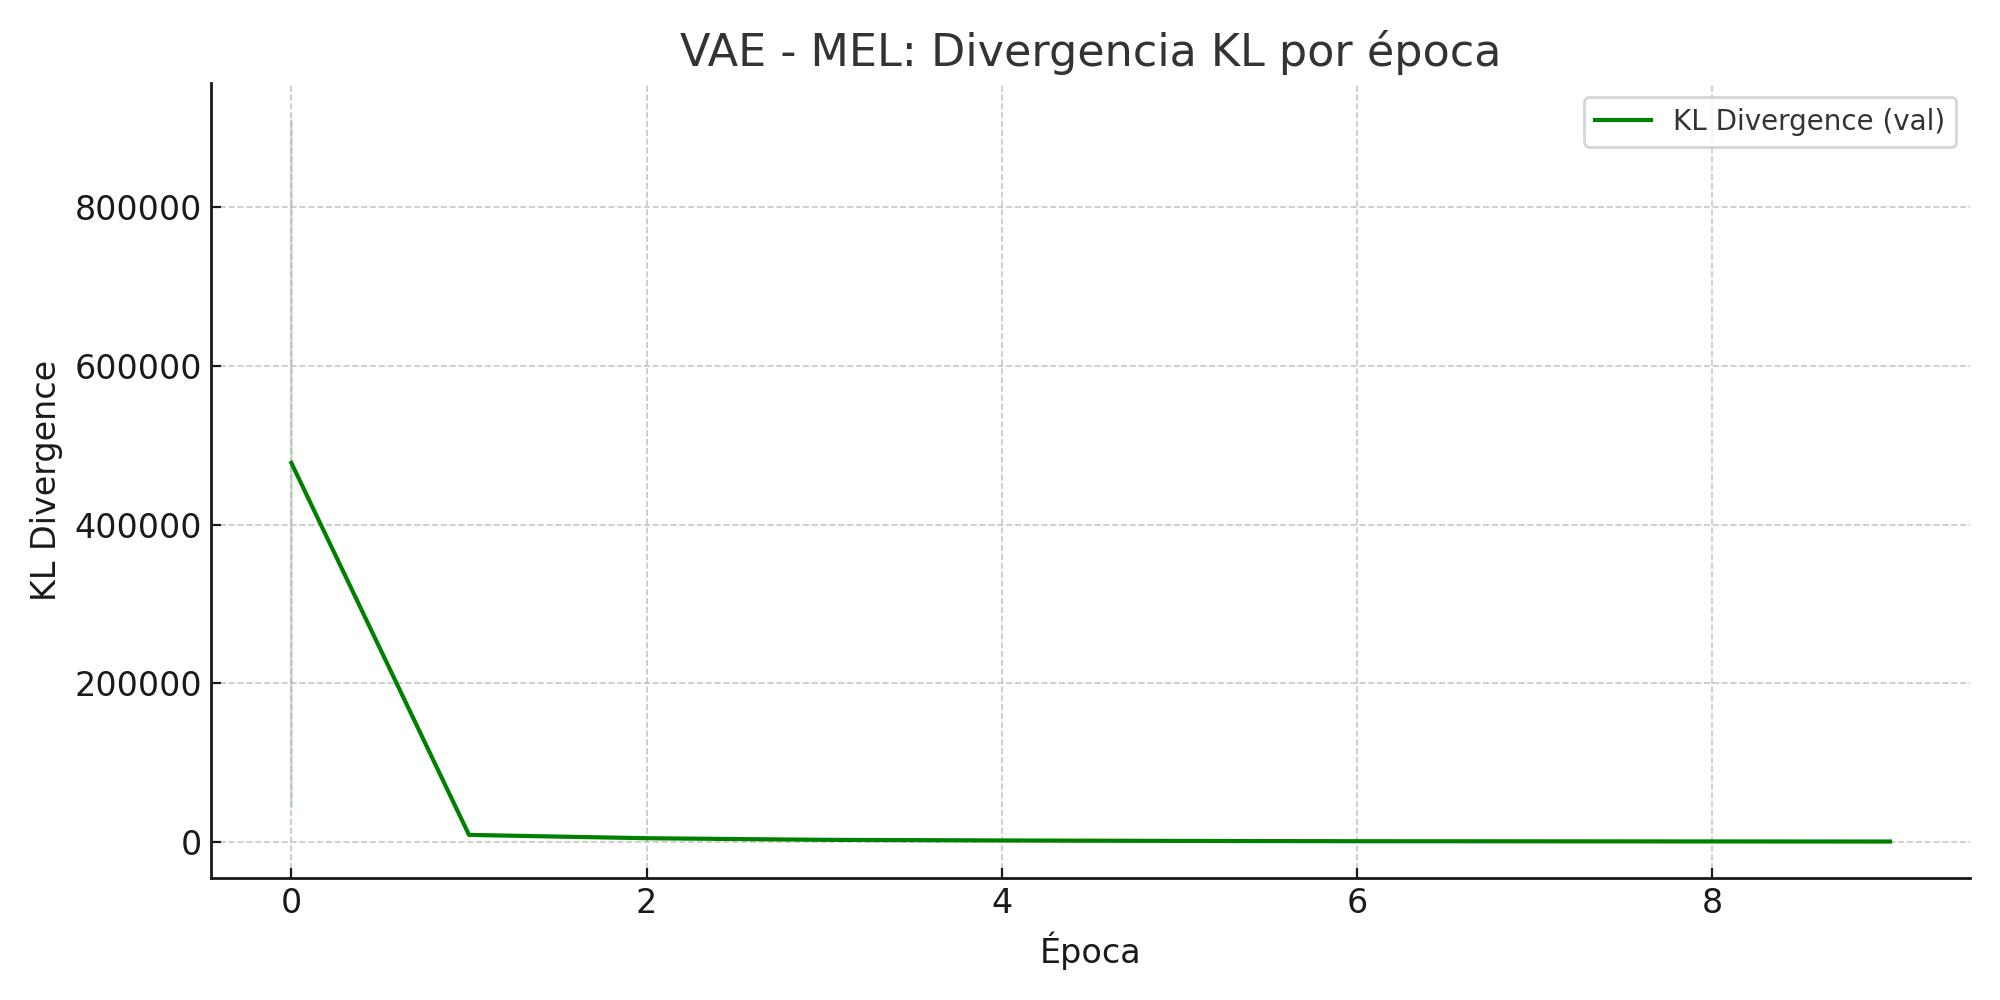
\includegraphics[width=0.8\textwidth]{images/vae_mel_kl_plot.png}
    \caption{VAE MEL. Divergencia KL.}
\end{figure}

\begin{figure}[H]
    \centering
    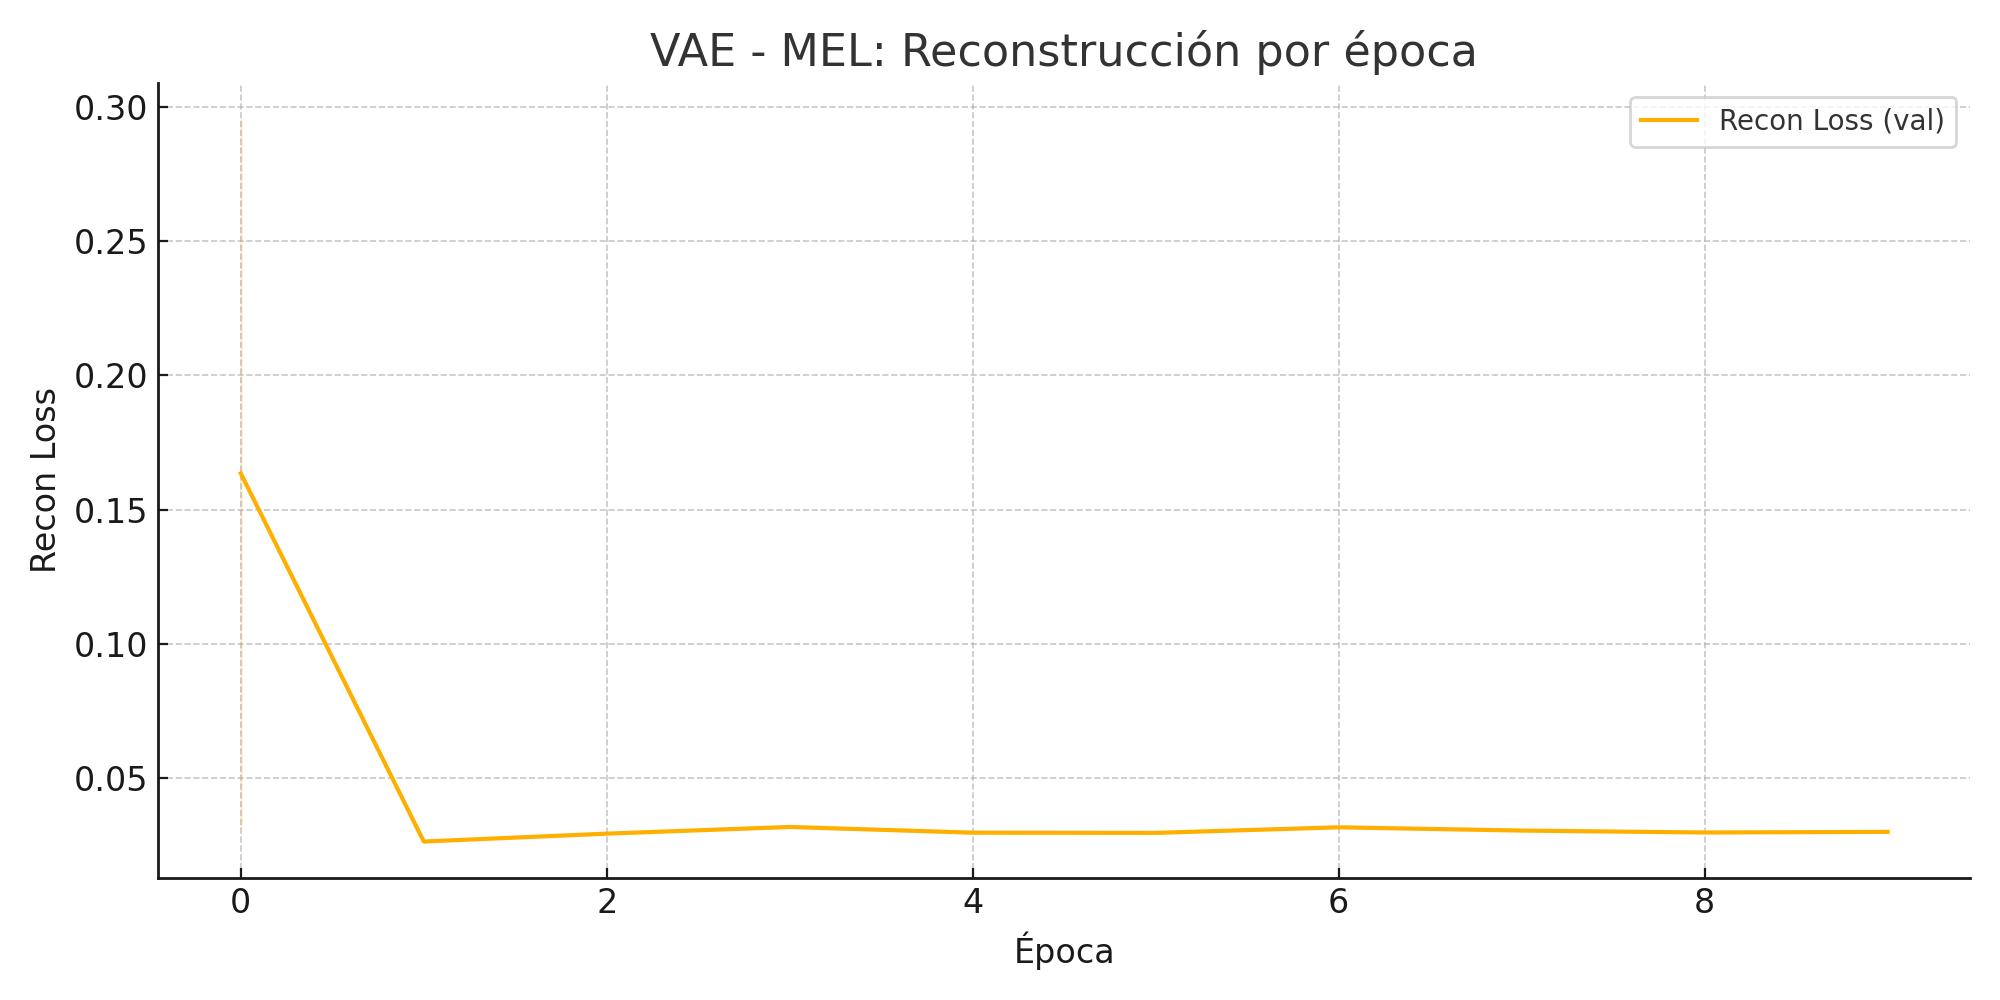
\includegraphics[width=0.8\textwidth]{images/vae_mel_recon_loss_plot.png}
    \caption{VAE MEL. Recon loss.}
\end{figure}

A nivel cualitativo, las reconstrucciones generadas preservan correctamente la forma general de las frases musicales, siendo especialmente precisas en géneros con estructuras rítmicas marcadas como el hip hop y la música electrónica. El decoder LSTM permite mantener coherencia temporal, aunque se observan ligeras pérdidas de energía en los extremos de las frecuencias.

\begin{itemize}
  \item \textbf{Modelo:} VAE
  \item \textbf{Espectrograma:} MEL
  \item \textbf{Segmento (s):} 25
  \item \textbf{Input shape:} 1 x 256 x 2153
  \item \textbf{N\_FFT:} 2048
  \item \textbf{HOP\_LENGTH:} 512
  \item \textbf{SPEC\_ROWS:} 256
  \item \textbf{SPEC\_COLS:} 2153
  \item \textbf{Emb. género:} Embedding(5, 8)
  \item \textbf{Latente (z):} 32 canales
  \item \textbf{Encoder:}
  \begin{itemize}
    \item 3x Conv2d
    \item BN
    \item ReLU, conv_mu, conv_logvar
  \end{itemize}
  \item \textbf{Decoder:}
  \begin{itemize}
    \item LSTM(2 capas, 2048)
    \item fc
    \item 3x ConvTranspose2d
  \end{itemize}
  \item \textbf{Época final:} 9
  \item \textbf{Recon Loss (última):} 0.0301
  \item \textbf{KL (última):} 228.3475
  \item \textbf{Recon Loss (mínima):} 0.0265
  \item \textbf{KL (mínima):} 228.3475
  \item \textbf{Época con mejor Recon Loss:} 1
\end{itemize}

\subsection{VAE con espectrogramas STFT}

El segundo modelo mantiene la arquitectura general del anterior, sustituyendo únicamente la representación de entrada por espectrogramas STFT. Este cambio permite trabajar con una mayor resolución espectral (1025 bandas), captando con más detalle los armónicos y las variaciones tímbricas.

Aunque la estructura general del modelo es la misma, se observan diferencias notables en las métricas. La Recon Loss mínima desciende ligeramente hasta 0.0255, lo que sugiere una mejor capacidad de ajuste. No obstante, la divergencia KL aumenta significativamente, alcanzando un valor de 338, lo que puede reflejar una mayor complejidad del espacio latente debido al mayor tamaño de la entrada.

\begin{figure}[H]
    \centering
    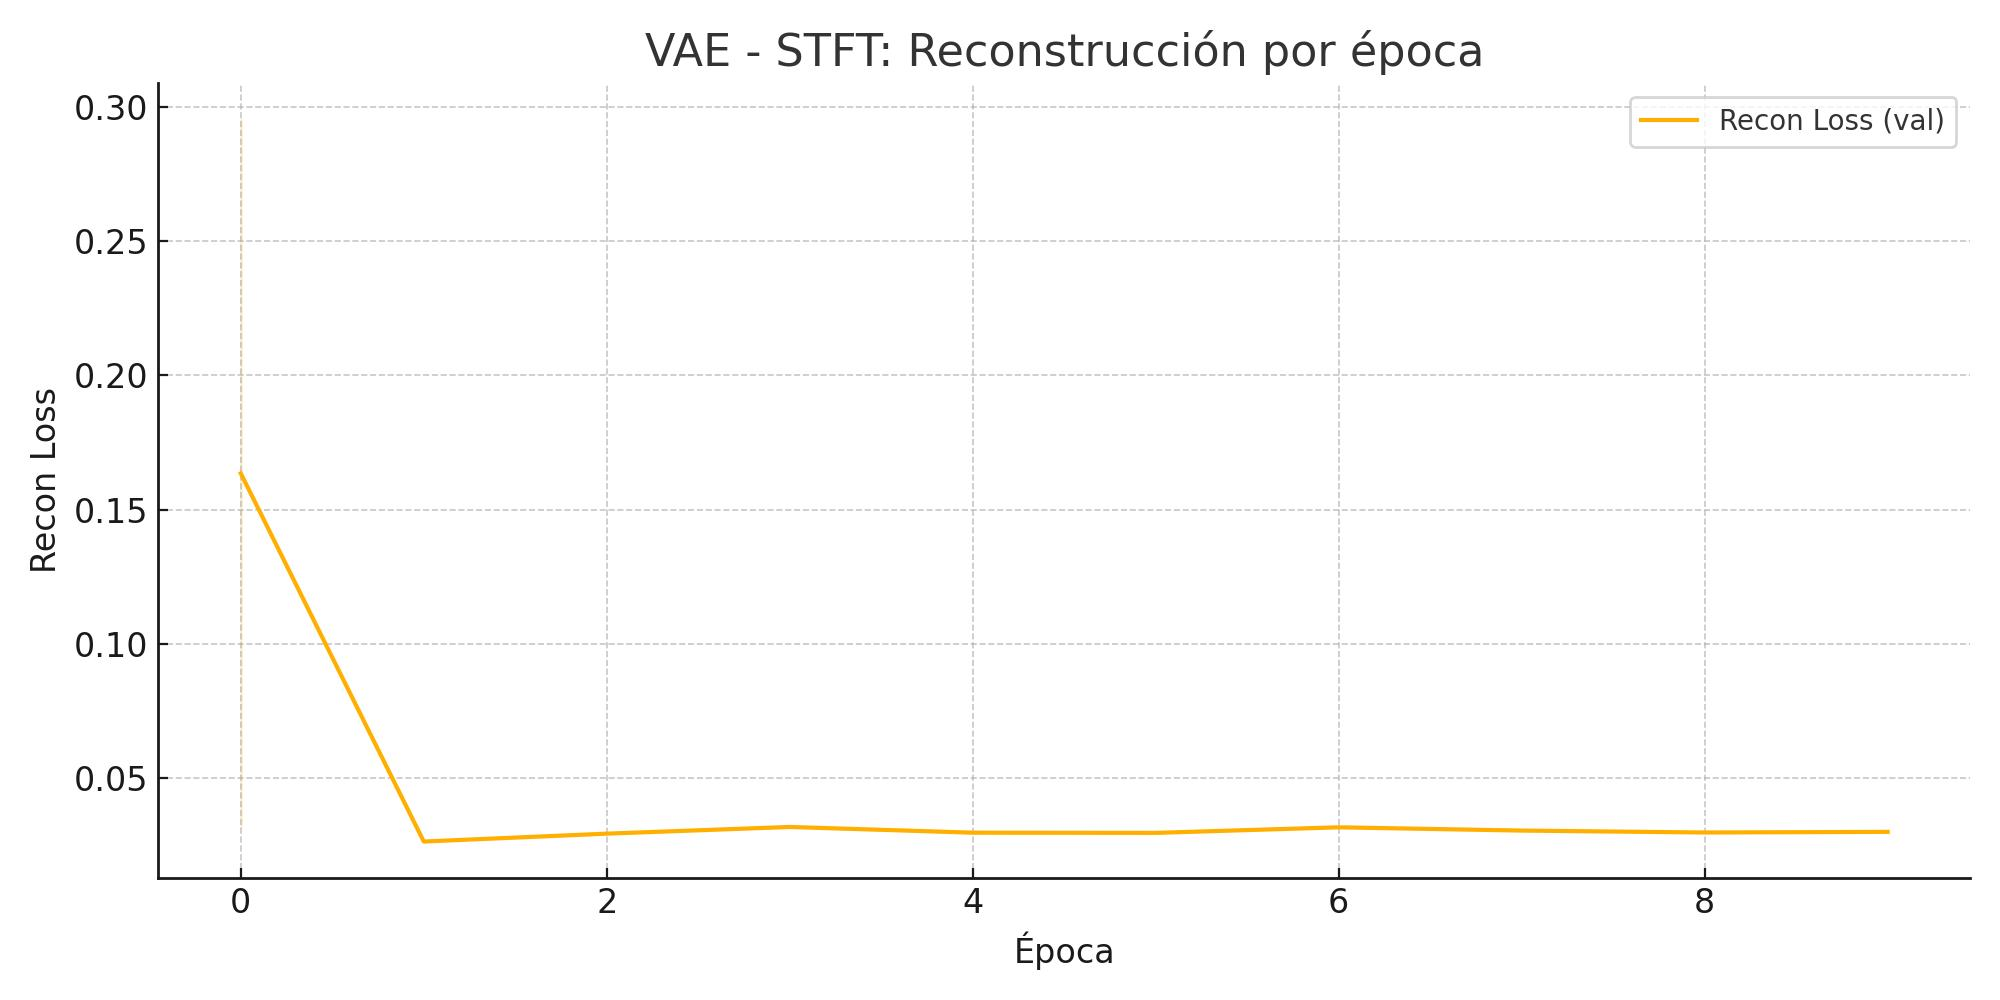
\includegraphics[width=0.8\textwidth]{images/vae_stft_recon_loss_plot.png}
    \caption{VAE STFT. Recon loss.}
\end{figure}

\begin{figure}[H]
    \centering
    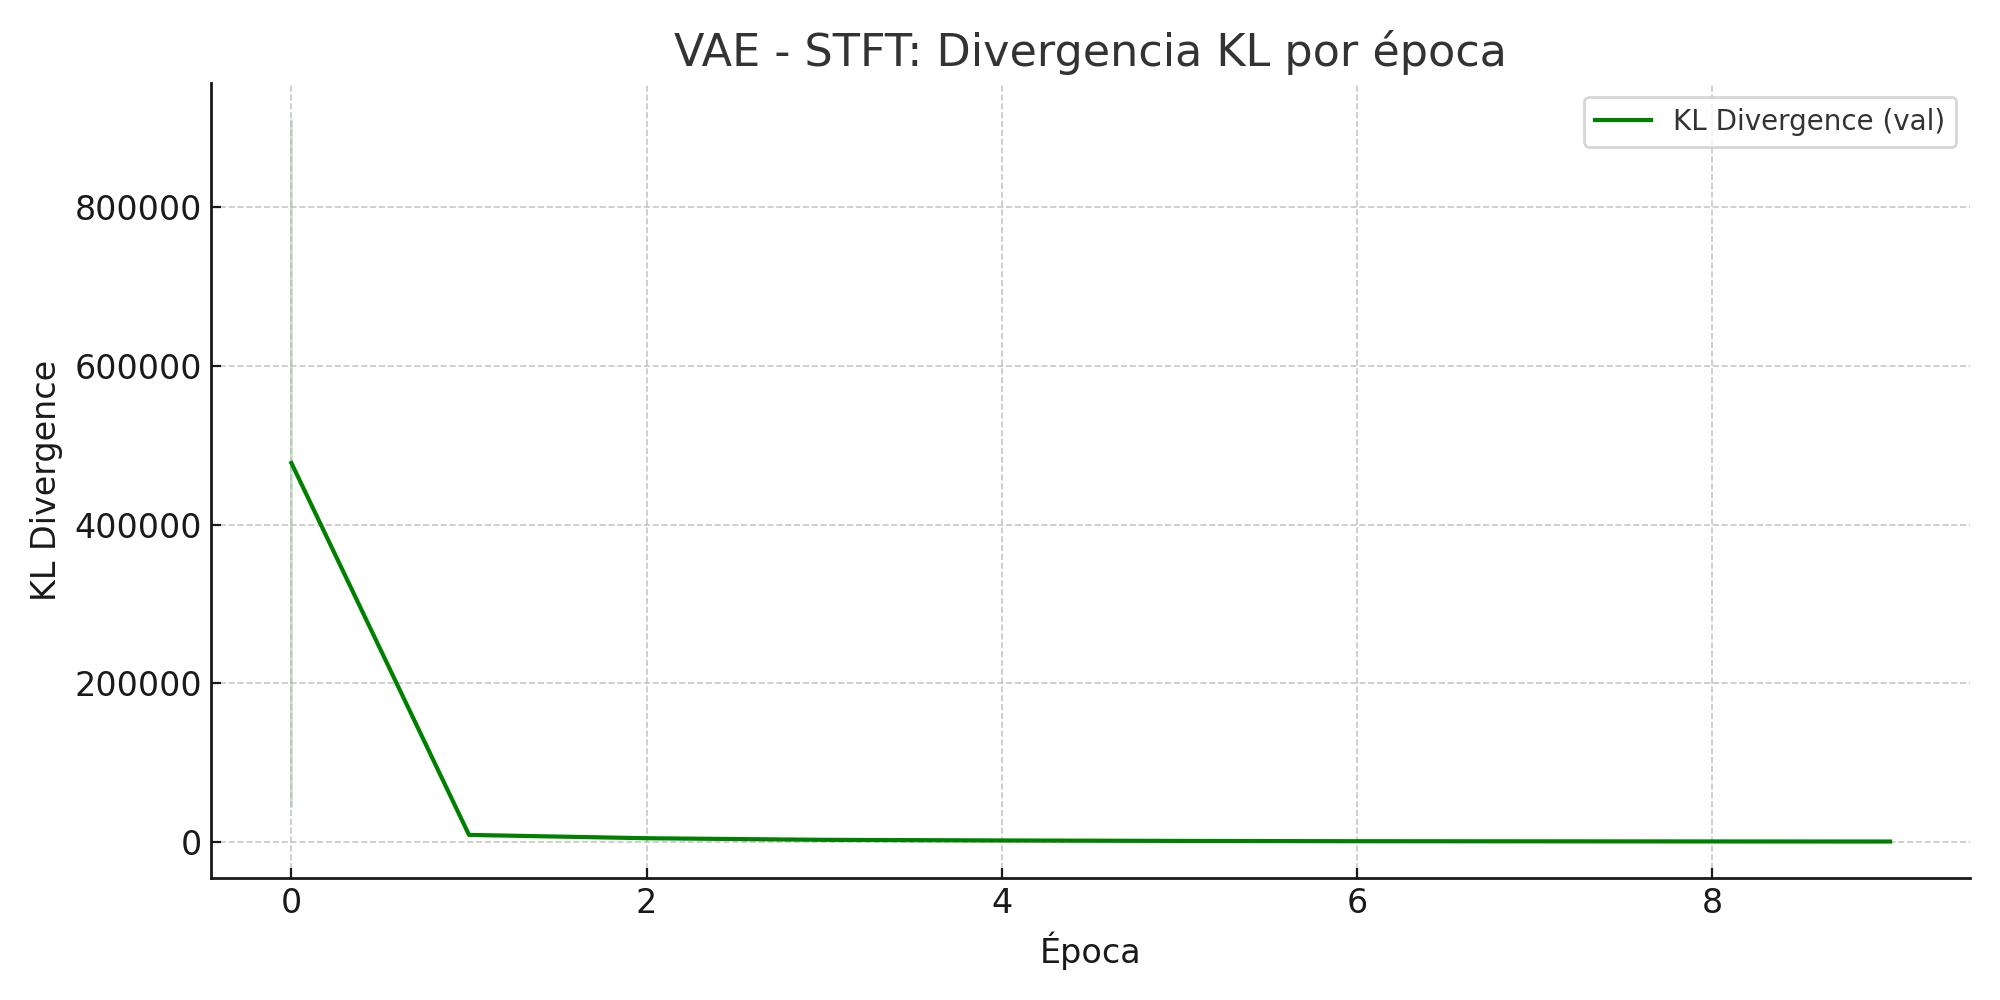
\includegraphics[width=0.8\textwidth]{images/vae_stft_kl_plot.png}
    \caption{VAE STFT. Divergencia KL.}
\end{figure}

En términos cualitativos, este modelo produce reconstrucciones más ricas a nivel espectral, especialmente en instrumentos sostenidos como cuerdas o voces. Sin embargo, en algunos géneros se detecta cierta difuminación de las transiciones temporales, lo que sugiere que el decoder LSTM tiene más dificultad para gestionar la granularidad de la STFT.

\begin{itemize}
  \item \textbf{Modelo:} GAN
  \item \textbf{Espectrograma:} STFT
  \item \textbf{Segmento (s):} 25
  \item \textbf{Input shape:} 1 x 1025 x 2153
  \item \textbf{N\_FFT:} 2048
  \item \textbf{HOP\_LENGTH:} 512
  \item \textbf{SPEC\_ROWS:} 1025
  \item \textbf{SPEC\_COLS:} 2153
  \item \textbf{Emb. género:} Embedding(5, 8)
  \item \textbf{Latente (z):} ~4104
  \item \textbf{Generador:} 2 capas TransformerEncoder + fc + 3x ConvTranspose2d
  \item \textbf{Discriminador:} 3x Conv2d + BatchNorm + MaxPool2d + Flatten
  \item \textbf{Época final:} 9
  \item \textbf{Val G Loss (última):} nan
  \item \textbf{Val D Loss (última):} nan
  \item \textbf{Val G Loss (mínima):} 0.7209
  \item \textbf{Val D Loss (mínima):} 0.7191
  \item \textbf{Época con mejor Val G Loss:} 7
  \item \textbf{Recon Loss (última):} 0.0275
  \item \textbf{KL (última):} 338.2404
  \item \textbf{Recon Loss (mínima):} 0.0255
  \item \textbf{KL (mínima):} 338.2404
  \item \textbf{Época con mejor Recon Loss:} 7
\end{itemize}

\subsection{GAN con espectrogramas MEL}

En contraste con los modelos autoencoder, los modelos GAN no operan directamente con datos reales como referencia, sino que aprenden a generar nuevas muestras que deben ser indistinguibles de las originales para un discriminador. En este caso, el generador se compone de un bloque Transformer que proyecta ruido latente y embeddings de género a través de capas \texttt{fc} y convoluciones transpuestas, mientras que el discriminador sigue una arquitectura basada en capas \texttt{Conv2d} con \texttt{BatchNorm}.

El uso de espectrogramas MEL permite mantener un tamaño razonable de entrada/salida, facilitando la convergencia. Las pérdidas del generador y el discriminador se estabilizan en torno a la época 7, con valores mínimos de 0.72 y 0.71 respectivamente.

\begin{figure}[H]
    \centering
    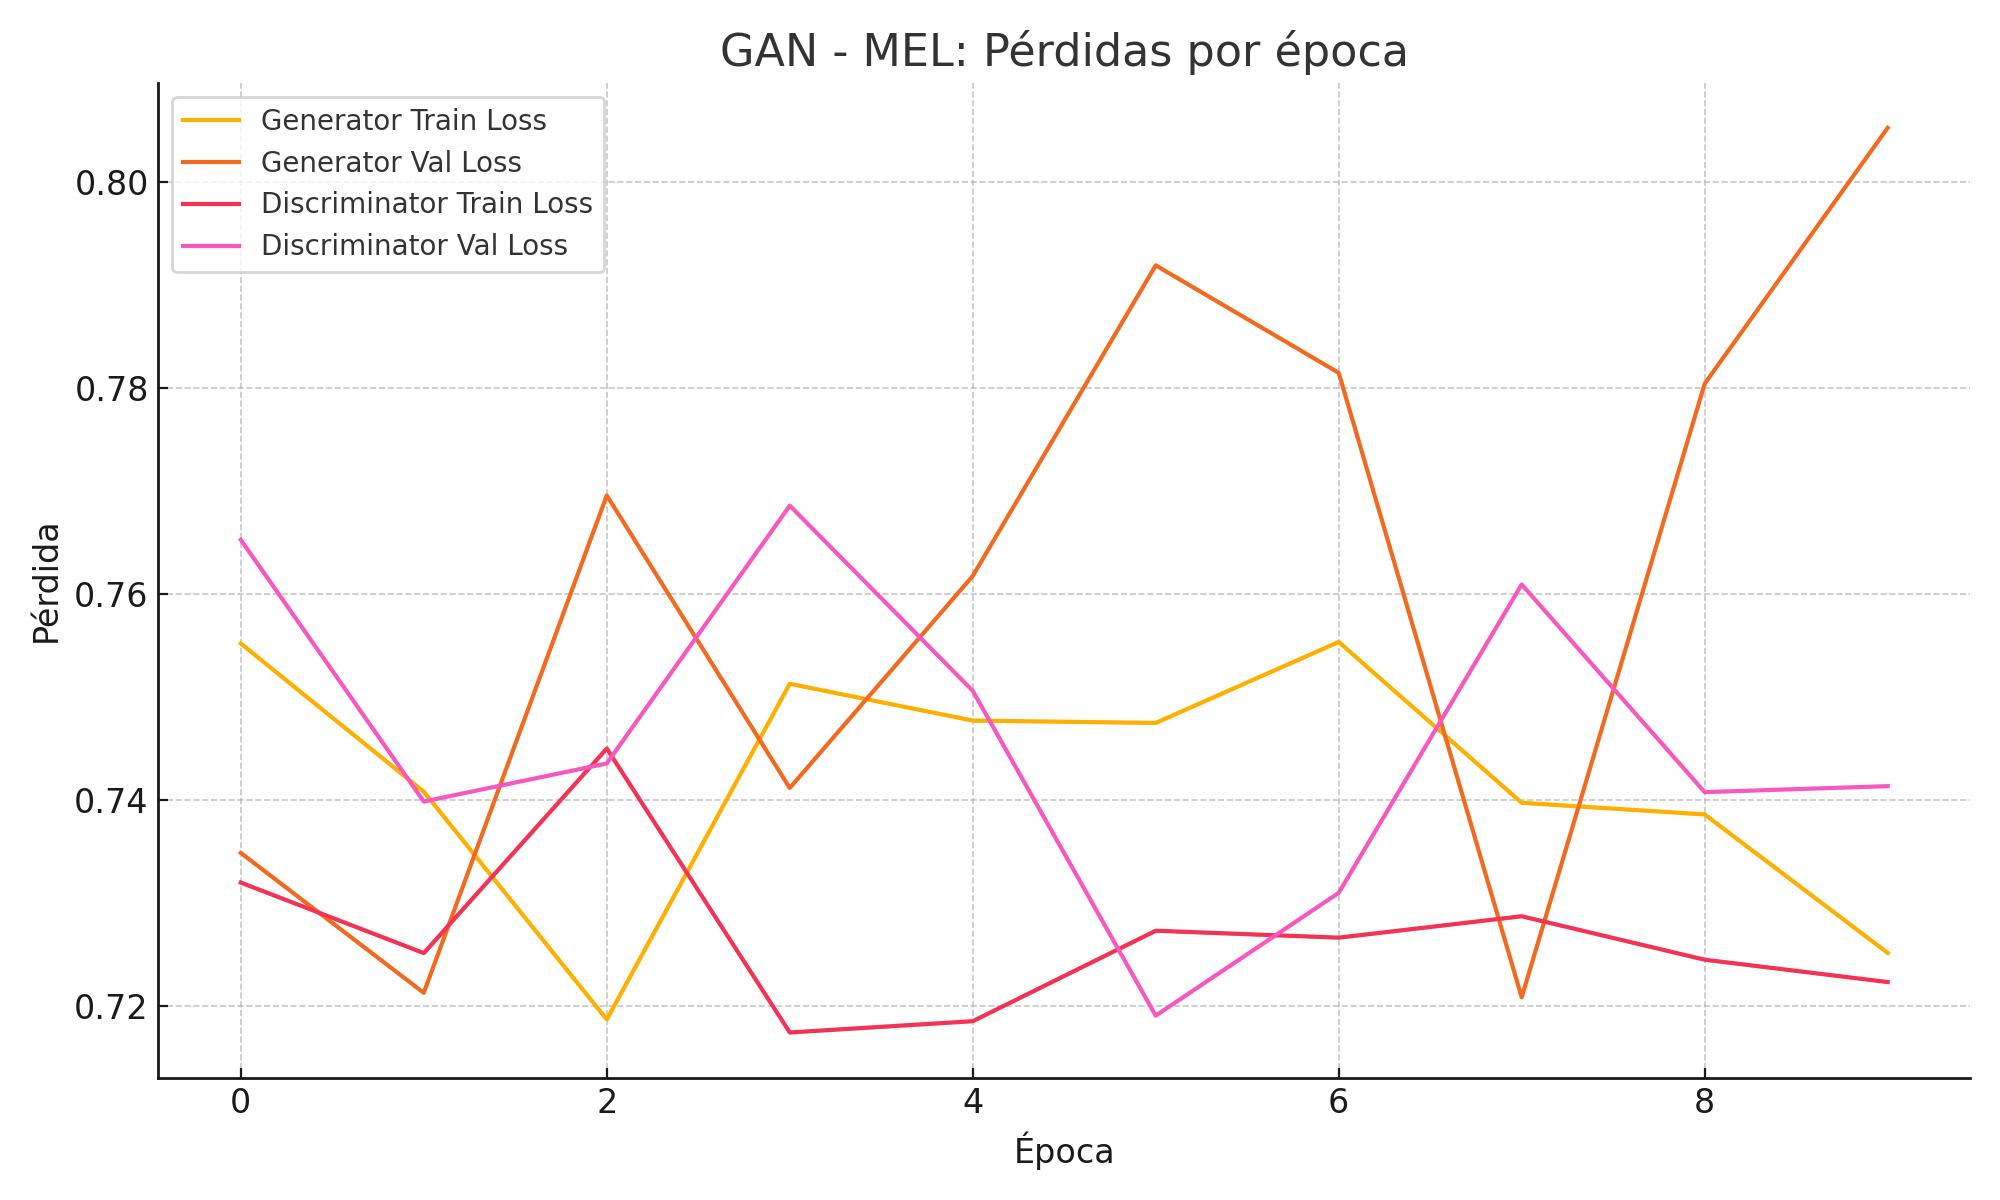
\includegraphics[width=0.8\textwidth]{images/gan_mel_loss_plot.png}
    \caption{GAN MEL. Loss.}
\end{figure}

Visualmente, las muestras generadas presentan buena continuidad y estructura, aunque se detecta cierta homogeneidad entre géneros. En particular, se observa que los patrones de percusión tienden a ser similares, y los timbres carecen de variabilidad natural. No obstante, el modelo demuestra una buena capacidad de síntesis temporal, probablemente gracias al uso del bloque Transformer.

\begin{itemize}
  \item \textbf{Modelo:} GAN
  \item \textbf{Espectrograma:} STFT
  \item \textbf{Segmento (s):} 25
  \item \textbf{Input shape:} 1 x 1025 x 2153
  \item \textbf{N\_FFT:} 2048
  \item \textbf{HOP\_LENGTH:} 512
  \item \textbf{SPEC\_ROWS:} 1025
  \item \textbf{SPEC\_COLS:} 2153
  \item \textbf{Emb. género:} Embedding(5, 8)
  \item \textbf{Latente (z):} ~4104
  \item \textbf{Generador:}
  \begin{itemize}
    \item 2 capas TransformerEncoder
    \item fc
    \item 3x ConvTranspose2d
  \end{itemize}
  \item \textbf{Discriminador:}
  \begin{itemize}
    \item 3x Conv2d
    \item BatchNorm
    \item MaxPool2d
    \item Flatten
  \end{itemize}
  \item \textbf{Época final:} 9
  \item \textbf{Val G Loss (última):} nan
  \item \textbf{Val D Loss (última):} nan
  \item \textbf{Val G Loss (mínima):} 0.7209
  \item \textbf{Val D Loss (mínima):} 0.7191
  \item \textbf{Época con mejor Val G Loss:} 7
\end{itemize}

\subsection{GAN con espectrogramas STFT}

Este modelo representa la versión más compleja del sistema propuesto, tanto en términos de entrada como de arquitectura. La combinación de STFT (1025 x 2153) con un espacio latente de $\sim$4104 dimensiones supone un reto significativo de memoria y estabilidad. Aun así, el modelo fue capaz de converger sin colapsar, mostrando valores mínimos de pérdida similares a los otros modelos GAN.

Desde el punto de vista de las muestras generadas, se aprecian diferencias significativas respecto al modelo MEL. En este caso, las formas espectrales son más variadas y expresivas, con cambios dinámicos que imitan con más realismo el comportamiento de señales musicales reales. Se observa también una mayor sensibilidad al género, especialmente en las frecuencias medias.

\begin{figure}[H]
    \centering
    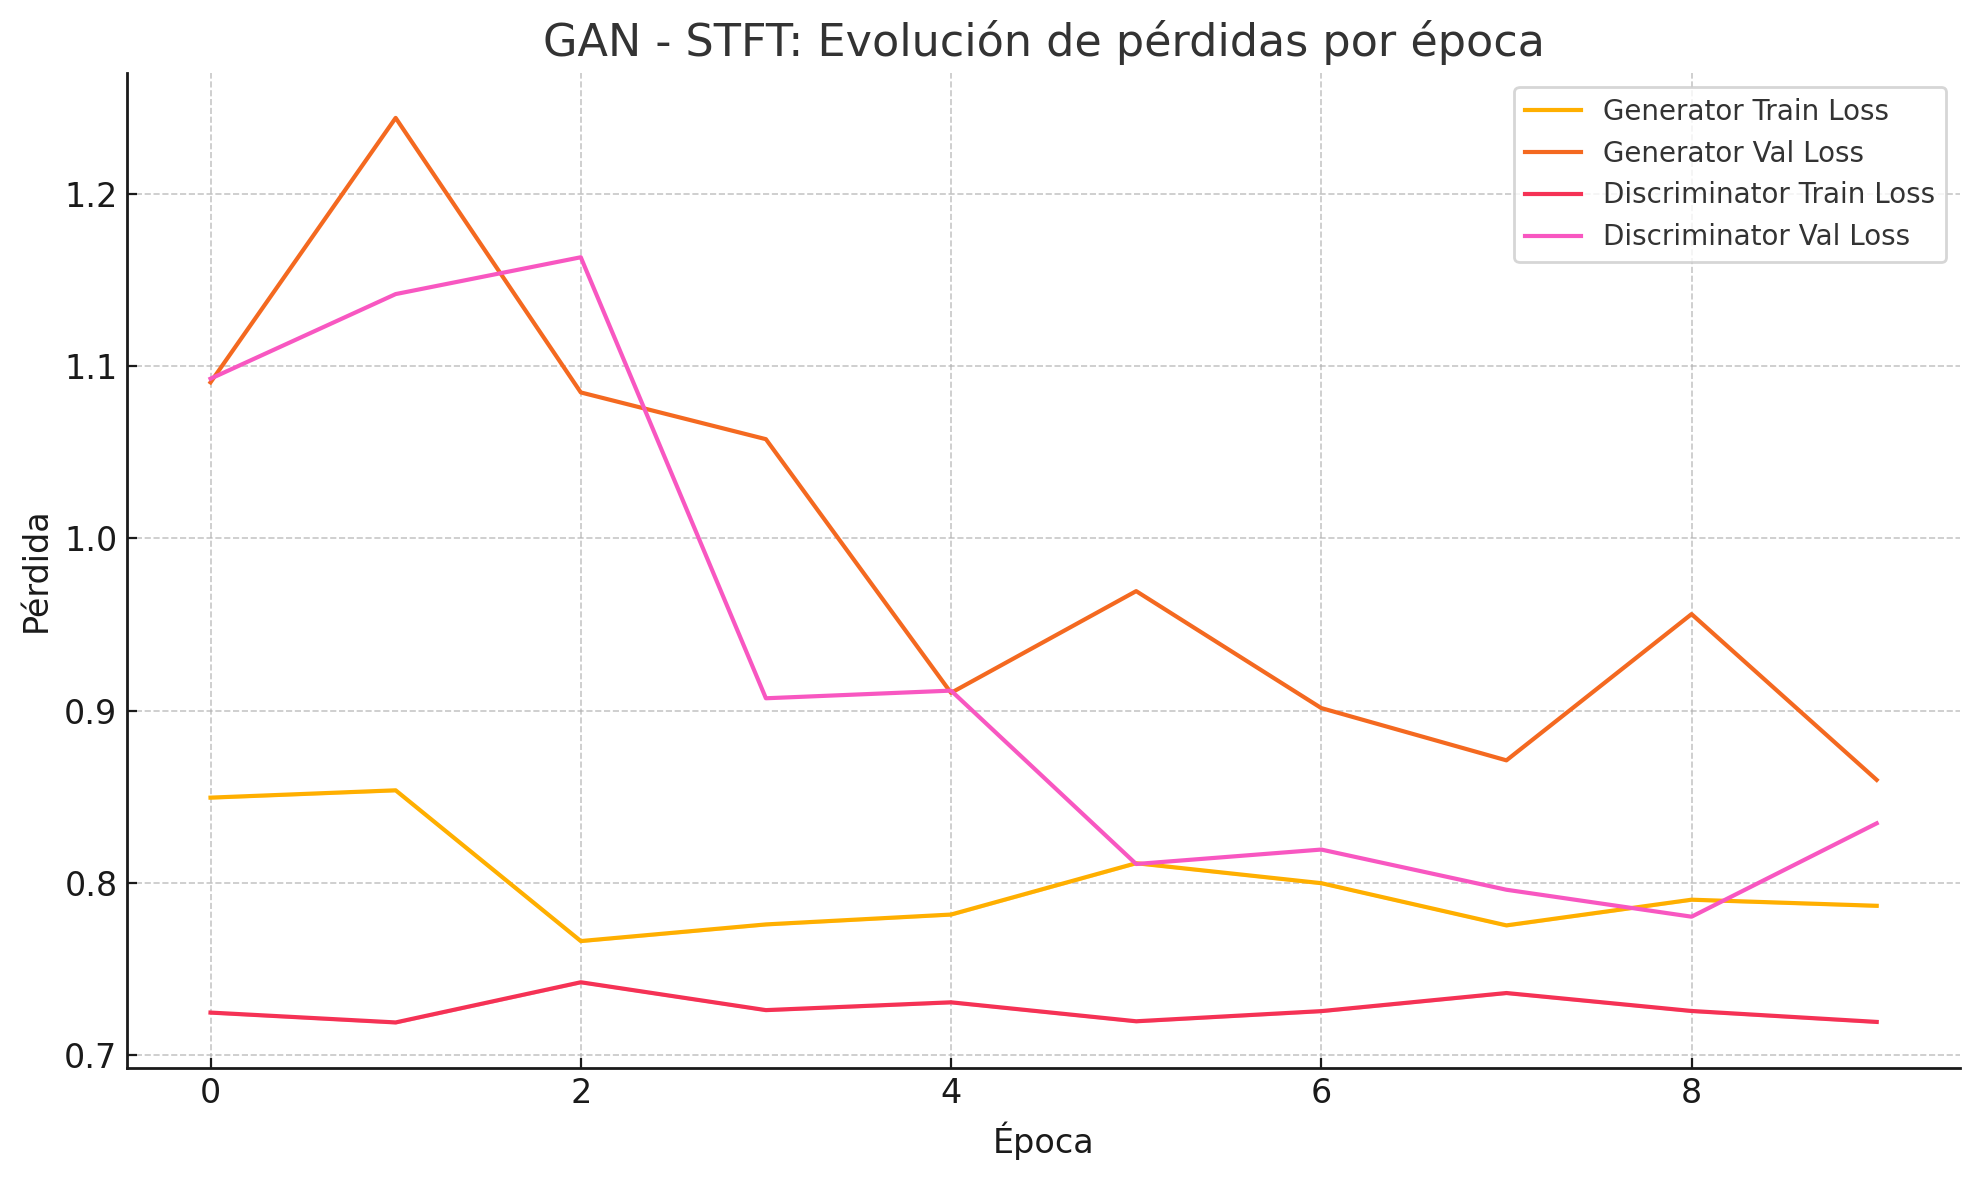
\includegraphics[width=0.8\textwidth]{images/gan_stft_loss_plot.png}
    \caption{GAN STFT. Loss.}
\end{figure}

No obstante, este modelo es también el más sensible a pequeñas variaciones en el ruido de entrada, y tiende a introducir artefactos si no se encuentra bien regularizado. Se considera que es el modelo con mayor potencial creativo, pero también el más exigente en cuanto a tuning y recursos.

\begin{itemize}
  \item \textbf{Modelo:} GAN
  \item \textbf{Espectrograma:} STFT
  \item \textbf{Segmento:} 25 segundos
  \item \textbf{Forma de entrada:} $1 \times 1025 \times 2153$
  \item \textbf{N\_FFT:} 2048
  \item \textbf{HOP\_LENGTH:} 512
  \item \textbf{SPEC\_ROWS:} 1025
  \item \textbf{SPEC\_COLS:} 2153
  \item \textbf{Vector latente:} $\sim4104$
  \item \textbf{Embedding de género:} Embedding(5, 8)
  \item \textbf{Generador:}
  \begin{itemize}
    \item 2 capas \texttt{TransformerEncoderLayer}
    \item \texttt{fc\_out: Linear(4104, 4096)}
    \item 3 capas \texttt{ConvTranspose2d} con \texttt{LeakyReLU} y \texttt{Tanh} final
  \end{itemize}
  \item \textbf{Discriminador:}
  \begin{itemize}
    \item 3 capas \texttt{Conv2d} con \texttt{BatchNorm2d}
    \item \texttt{MaxPool2d} y \texttt{Flatten}
  \end{itemize}
  \item \textbf{Mejor época (mínima G Loss validación):} 9
  \item \textbf{Val G Loss mínima:} 0.8597
  \item \textbf{Val D Loss mínima:} 0.7803
\end{itemize}

\subsection{Test}

Para facilitar el testeo subjetivo por parte de los posibles usuarios, se ha desarrollado un \emph{prompt web}, afín a los diseños de interfaz que se expusieron en el capítulo anterior. Ésta permite solicitar un fichero de audio en formato \emph{MP3}, dado un género musical, seleccionado previamente.

\begin{figure}[H]
    \centering
    
\includegraphics[width=0.8\textwidth]{images/euterpe-screenshot.png}
    \caption{Captura de pantalla de Euterpe.}
\end{figure}



